\documentclass{article}
\usepackage{amsmath}
\usepackage{amssymb}
\usepackage{graphicx}
\usepackage{enumitem}
\usepackage[utf8]{inputenc}
\graphicspath{{Imagenes/}}

\title{\Huge Taller de Herramientas Computacionales}
\author {Diego Armando Santillán Arriaga}
\date{15/enero/19}
	
\begin{document}
\maketitle
	\begin{center}
		%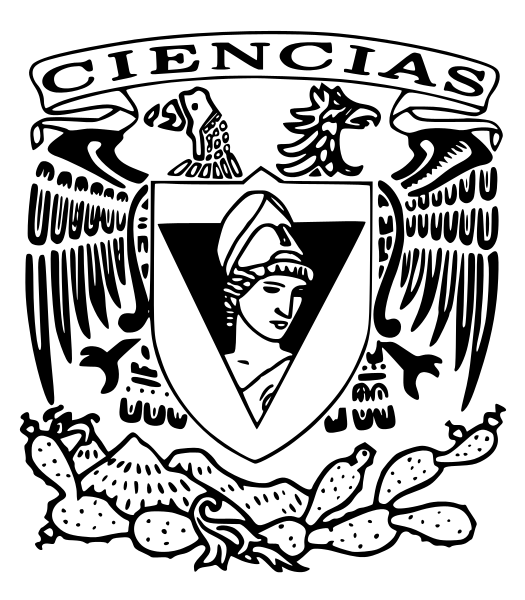
\includegraphics[scale=0.40]{1.png}
	\end{center}
\newpage

%\section{Expresiones matemáticas}: sin asterisco aparece el número de sección.
\section*{Expresiones matemáticas}
$\alpha + \beta$\\ %\(\)
\[\alpha + \beta\] %Con corchetes se centra el texto en la línea siguiente

\subsection{Índices y subíndices}
$x_{2}$
$x^2$

\end{document}
